\begin{table}[h]
  \small
  \centering
  \begin{tabular}{c c c c}
    \toprule
    Application & Knobs & Utility & Dataset \\
    \midrule
    \specialcell{Pedestrian\\Detection}
                & \specialcell{resolution \\ frame rate \\ quantizer }
                & F1 score & \specialcell{training: MOT16-04\\testing: MOT16-03} \\
    \midrule
    \specialcell{Augmented\\Reality}
                & \specialcell{resolution \\ frame rate \\ quantizer }
                & F1 score & \specialcell{training: office video\\testing: home
    video} \\
    \midrule
    \specialcell{Top-k}
                & \specialcell{head (N) \\ threshold (T) }
                & \specialcell{Kendall's $\tau$}
                & \specialcell{sec.gov access log \\ training: 4 days \\
    testing: 16 days} \\
    \bottomrule
  \end{tabular}
  \caption{\sysname{} Applications}
  \label{tab:apps}
\end{table}

\section{Implementation}
\label{sec:implementation}

In this section we present details about our implementation, including a
prototype framework and three non-trivial wide-area streaming applications.
\sysname{} is implemented in Rust and open-source on Github.\footnote{Url elided
  for anonymity.}

\subsection{Framework}
\label{sec:framework}

While our proposed APIs are general and not language specific, we chose a safe
language, Rust, for the core framework for the following reasons.

% First, Rust's memory safety guarantee can ensure applications running
% continously for an extended period of time. Besides, the zero-cost abstraction
% removes the possibilities of tail latencies caused by uncoordinated garbage
% collection~\cite{maas2016taurus}. In addition, we rely on Rust's type system to
% enforce the type match on \texttt{maybe} operations.

% All operators implement the \texttt{Stream} trait which has an associate type
% \texttt{Item} and a core function \texttt{next} that returns
% \texttt{Datum}. Each datum is either an item with the \texttt{Stream::Item} or
% an \texttt{Error} that the operator use to communicate with the runtime
% scheduler. The concrete form of \texttt{maybe} API is almost an direct
% translation of the API specification. While our API specification
% in~\autoref{tab:operators} uses a vector for knobs, our Rust implementation is
% more general: any type (including vector) that implements \texttt{IntoKnob}
% trait can be used as the knob.
% \begin{lstlisting}
% pub trait Stream {
%     type Item;
%     fn next(&mut self) -> Datum<Self::Item, Error>;

%     fn maybe<K, F>(self, opts: K, f: F) -> Maybe<Self, F>
%         where Self: Sized,
%                 K: IntoKnob,
%                 F: FnMut(K::Item, Self::Item) -> Self::Item {

%          // omitted
%     }
% }
% \end{lstlisting}

Applications built with \sysname{} runs as a single process. The entire
processing pipeline is often specified in a single main file. The execution mode
(profiling, runtime as client or runtime as server) is configured with command
line arguments or environment variables. Our deployment manager is currently a
shell script.

\subsection{Building \sysname{} Applications}
\label{sec:build-appl}

Using \sysname{}, we've built three applications: pedestrian detection
surveillance, an augmented reality and a distributed Top-k. \autoref{tab:apps}
summarizes the application specific part: knobs, utility function and dataset

% \begin{figure*}
%   \centering
%   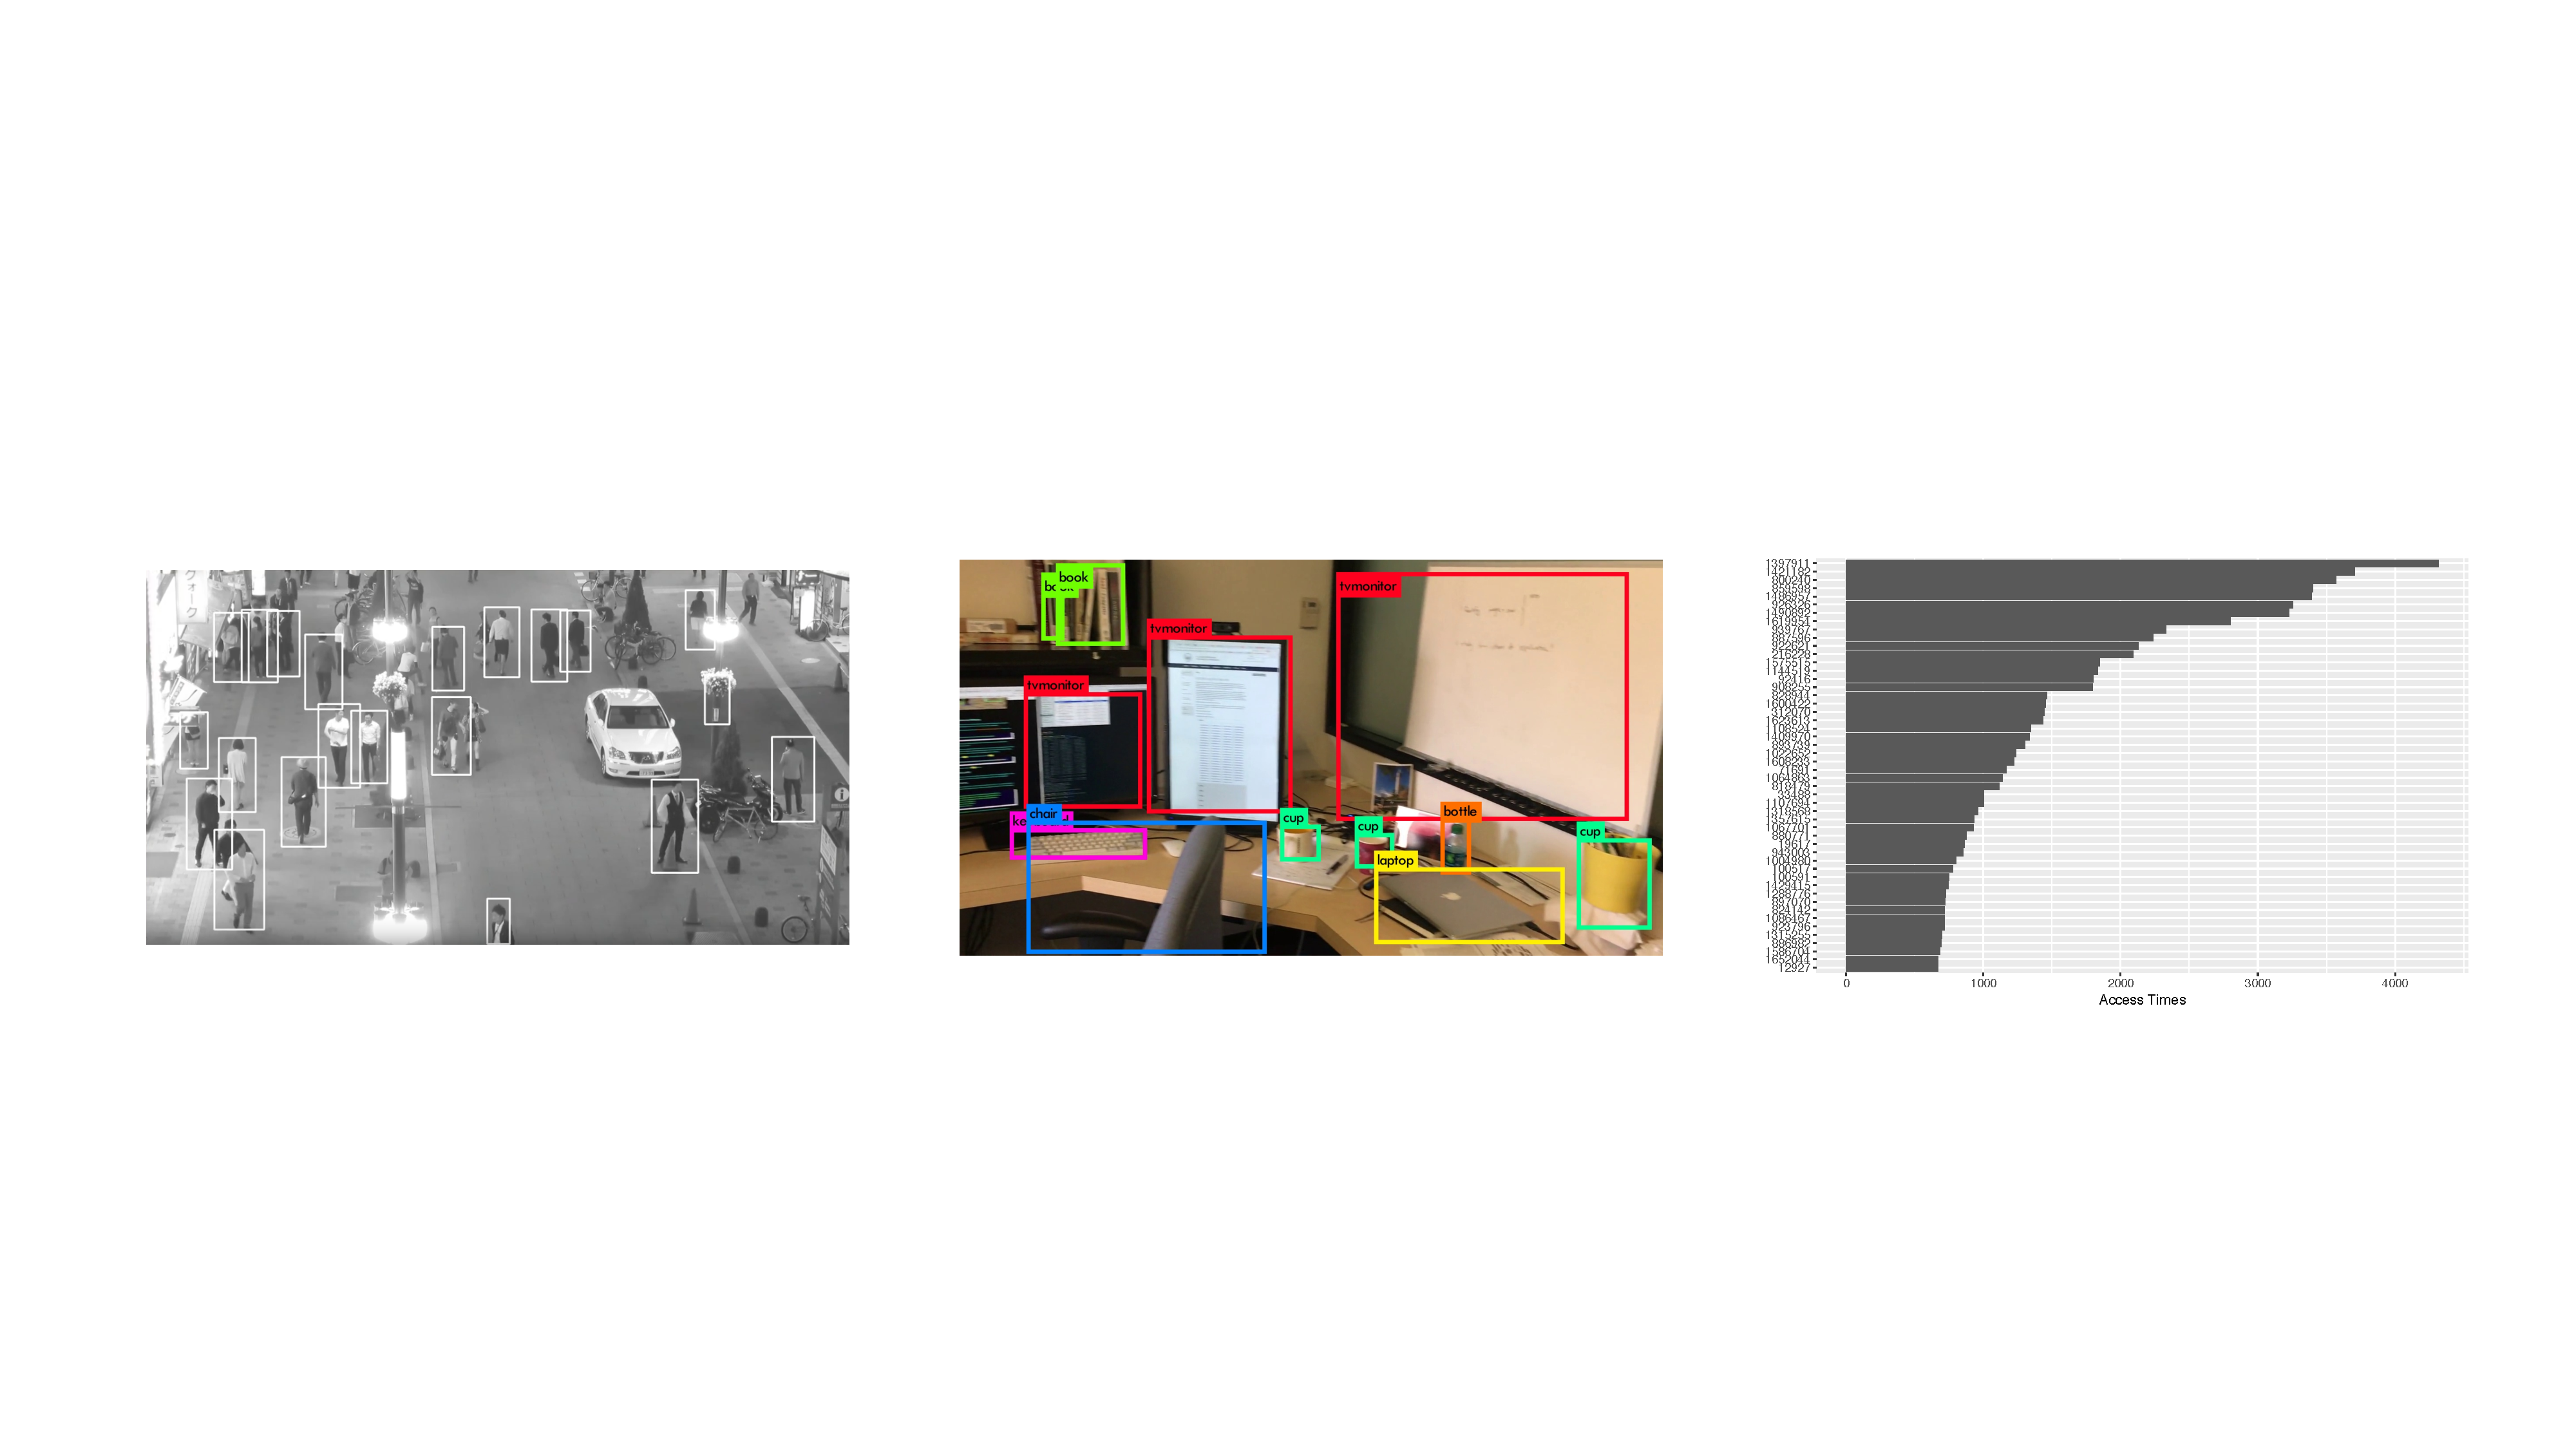
\includegraphics[width=\textwidth]{figures/apps.pdf}
%   \caption{Applications}
%   \label{fig:apps}
% \end{figure*}

\para{Pedestrian Detection:} This application analyzes video streams from
installed CCTV cameras and detect pedestrians inside. We implement most
image-related operations with OpenCV 3.1~\cite{opencvlibrary}. Pedestrians are
detected using histogram of oriented gradients (HOG)~\cite{dalal2005histograms}
with the default linear SVM classifier. To ensure real-time processing of
frames, GPU-accelerated implementation is used in favor of the CPU-based
implementation. For video encoding, H.264 scheme is chosen for its prevalence in
existing systems. Our implemenation is based on GStreamer~\cite{gstreamer},
using \texttt{x264enc} plugin. To integrate with \sysname{}, we first create a
pipeline that exposes \texttt{appsrc} (to feed raw image data) and
\texttt{appsink} (to get encoded bytes). The GStreamer main loop is managed in a
separate thread and \sysname{} communicates with it via Rust's channel. The
\texttt{x264enc} is configured with \texttt{zerolatency} present and runs using
four threads. It uses constant quality encoding and the quantizer is exported as
a parameter that can be tuned.

The detection returns a list of bounding boxes; it's compared against a
reference result (either the groundtruth or the one without degradation). A
successful detection is defined when the intersection over union (IOU) is
greater than 50\%~\cite{everingham2010pascal}. For the utility function, we use
F1 score (\%), the harmonic mean of precision and
recall~\cite{Rijsbergen:1979:IR:539927}.

\para{Augmented Reality:} We target at mobile augmented reality applications
which offload the heavy computation to resources elsewhere. Although local
computation is gaining attraction~\cite{satyanarayanan2009case, zhang2015cloud},
wireless communication link is also susceptible to capacity variation.

We use a similar setup as the pedestrian detection application except the actual
function that analyzes the stream. To recognize objects, we use a a pre-trained
neural network~\cite{darknet13} that's trained with
Imagenet~\cite{krizhevsky2012imagenet}. Similar to our first application,
GPU-accelerated implementation is use in favor for real-time processing.

\para{Distributed Top-K:} Many monitoring applications require to answer the
``top-k'' question~\cite{babcock2003distributed}, such as the top-k most popular
URLs or the top-k most access files. Naively aggregating all the raw log entries
is not feasible as popular servers have millions of requests per second. Local
worker node can first perform a window-based transformation that generates data
summary, such as key-value pairs of \texttt{<item, count>}. However, even after
this operation, the data size could still be too large given most real-world
access patterns follow a long-tailed distribution. There is a
large-but-irrelevant tail that is unnecessary to send.

\begin{figure}
  \centering
  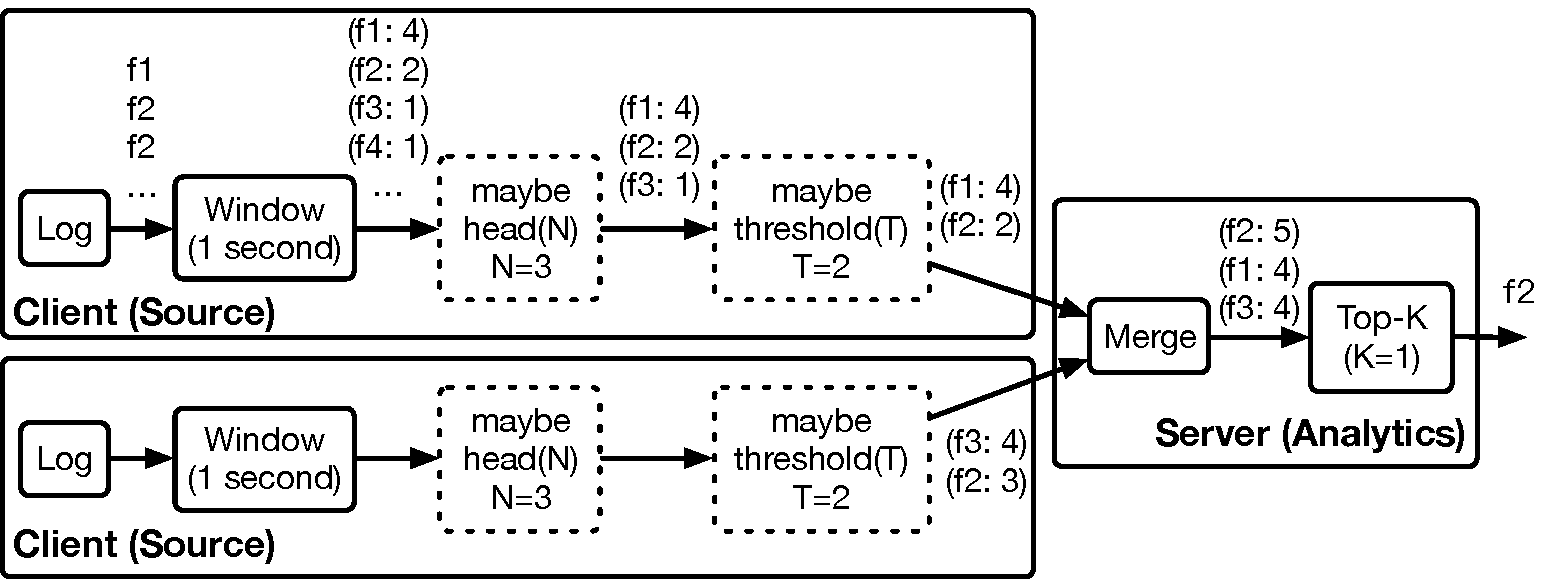
\includegraphics[width=\columnwidth]{figures/topk.pdf}
  \caption{Distributed Top-K Application}
  \label{fig:topk}
\end{figure}

We consider two degradation operations that individual worker nodes can perform:
(1) a head (\texttt{N}) operation that shortens the list first; (2) a threshold
\texttt{T} that further filters small entries. These two operations are not
orthognal to each other. Their impact on data size reduction and quality
degradation depends on the distribution of the actual data. We use Kendall's
$\tau$ as the utility function here. It is a correlation measure of the
concordance between two ranked list. The function outputs the rank correlation
ranging from -1 to 1, representing no agreement to complete aggrement,
respectively~\cite{abdi2007kendall}. To integrate with \sysname{}, we convert
the measure to the range of [0, 1].

%%% Local Variables:
%%% mode: latex
%%% TeX-master: "sosp17"
%%% End:
